% Chapter 2

\chapter{Matrix Approach} % Main chapter title

\label{Chapter4} % For referencing the chapter elsewhere, use \ref{Chapter2} 

%----------------------------------------------------------------------------------------
\section{Colbourn, Day, Nel}

\section{Harvey, Xu}

\subsection{Techniques used}



\subsubsection{Naive chain rule algorithm}

% % % % Some Macros 

\newcommand{\laplacian}[1][G]{\ensuremath{L_{#1}^{+}}}
\newcommand{\reffformula}[1][\laplacian]{\ensuremath{ (\chi_u - \chi_v)^T \  #1 \ (\chi_u - \chi_v) }}
\newcommand{\reff}[1][e]{\ensuremath{R_#1^{\text{eff}}}}
\newcommand{\proj}{\ensuremath{I - \frac{\textbf{1} \textbf{1}^T}{n}}}

\newcommand{\Mset}[2]{\ensuremath{\mathbb{M}_{#1 \times #2}}}

%  from https://tex.stackexchange.com/questions/39390/writing-a-limit-so-that-the-subscript-goes-directly-underneath

\newcommand{\Lim}[1]{\raisebox{0.5ex}{\scalebox{0.8}{$\displaystyle \lim_{#1}\;$}}}


\begin{algorithm}[H]
 \KwIn{$G = (V,E) \  \text{and} \  L_G^+$}
 \KwOut{Set of edges corresponding to a random spanning tree}
 
 \For{$e = (u,v) \in E$ }{
    $R_e^{\text{eff}} = (\chi_u - \chi_v)^T \ L_G^+ \ (\chi_u - \chi_v)$\;
  \eIf{$(X \sim \text{Bernoulli}(R_e^{\text{eff}})) = 1$} {
   Add edge $e$ to the spanning tree\;
   $G = G / e$\;
   }{
   $G = G \setminus e$ \;
  }
  Update $ L_G^+ $ \;
 }
 \caption{Sampling uniform spanning tree using chain rule}
\end{algorithm}

\subsection{Facts used}

\begin{HXf}[Woodbury matrix identity]
 Let $ M \in \mathbb{M}_{n \times n} , U \in \mathbb{M}_{n \times k}, V \in \mathbb{M}_{n \times k}$. Suppose $M$ is non-singular then $M + UV^T$ is non-singular $\iff \ I + V^T M^{-1} U$ is non-singular. If $M + UV^T$ is non-singular, then 
 $$ (M + UV^T)^{-1} = M^{-1} - \left( M^{-1} \cdot U \cdot (I + V^TM^{-1}U)^{-1} \cdot V^T \cdot M^{-1}\right) $$
\end{HXf}

\begin{proof}
 TODO
\end{proof}

\begin{HXf}
 For any $L \in \mathbb{M}_{n \times n}$ with $\text{ker}(L) = \text{span}(\textbf{1})$, we have $LL^+ = I - \frac{\textbf{1} \cdot \textbf{1}^T}{n}$ and $P := I - \frac{\textbf{1} \cdot \textbf{1}^T}{n}$ is called the \textbf{projection matrix}. 
\end{HXf}

\begin{HXf}[Sub-matrices]
For all the results below, $S$ denotes a index set and $S^c$ denotes it's complement.
 \begin{enumerate}
  \item For any $A,B \in \Mset{n}{n}, (A + B)_{S,S} = A_{S,S} + B_{S,S}$
  \item If $C = D \cdot E \cdot F$ then $C_{S,S} = D_{S,*} \cdot E \cdot F_{*,S}$
  \item For $A \in \Mset{m}{n}, B \in \Mset{n}{l}$ , If $A_{S^c, S^c} = 0$ or $B_{S^c, S^c} = 0$ then \\ $(AB)_{S,S} = A_{S,S} \cdot B_{S,S}$
  \item For any matrix $C$ where $C = D \cdot E \cdot F$ . If $D_{*, S^c} = 0$ and $F_{S^c, *} = 0$, then $C = D_{*, S} \cdot E_{S,S} \cdot F_{S,*}$
  \item $D = 
\begin{bmatrix}
M & 0 \\
0 & 0 \\
\end{bmatrix},
$ 
and $
E = 
\begin{bmatrix}
A & B \\
X & Y \\
\end{bmatrix}
$
where $M, A \in \Mset{n}{n}$ and If $(MA - I)$ is invertible Then,
$$ (DE - I)^{-1} = \begin{bmatrix}
(MA - I)^{-1} & (MA - I)^{-1} \cdot M \cdot B \\
0 & -I \\
\end{bmatrix}
$$
\begin{proof}
 $(DE - I)^{-1}$ can be computed using Shur's Complement(\cite{wiki:shur}) . 
 
 Suppse $N =  
\begin{bmatrix}
P & Q \\
R & S \\
\end{bmatrix}
$ and Shur's complement of block $S$ and $P$ is  $$N / S := P - QS^{-1}R \qquad N / P := S - RP^{-1}Q$$
Then $$N^{-1} = 
\begin{bmatrix}
P^{-1} + (P^{-1} Q (N/P)^{-1} R  P^{-1}) & -(P^{-1}Q(N/P)^{-1}) \\[0.3cm]
-((N/P)^{-1}RP^{-1}) & (N/P)^{-1} \\
\end{bmatrix}
$$
In our case $N = 
\begin{bmatrix}
MA - I & MB \\
0 & -I \\
\end{bmatrix}
$ and $(N/P) = -I$. From this it follows that $$N^{-1} = (DE-I)^{-1} = \begin{bmatrix}
(MA - I)^{-1} & (MA - I)^{-1} \cdot M \cdot B \\
0 & -I \\
\end{bmatrix}
$$
\end{proof}

 \end{enumerate}

\end{HXf}

\begin{HXf}
 Let $A, B \in \Mset{n}{n}$ with $B$ being symmetric PSD. Suppose $x$ is an eigenvector of $AB$ corresponding to eigenvalue $\lambda$. Then $\sqrt{B} x$ is an eigenvector of $\sqrt{B}A\sqrt{B}$ corresponding to eigenvalue $\lambda$ 
\end{HXf}

\begin{HXf}
 Let $G$ be a graph with $n$ vertices. Suppose $(\lambda_1, \lambda_2 \cdots \lambda_n)$ be the eigenvalues corresponding to the eigenvectors $(v_1, v_2 \cdots v_n) $ of the Laplacian of $G$ denoted as $L_G$. $L_G$ is symmetric PSD with $\lambda_1 = 0$ and $v_1 = \textbf{1}$. The following properties relate the eigenvalues of $L_G$ with the connectivity of $G$ :
 
\begin{enumerate}
 \item $\lambda_2 > 0 \iff G$ is connected
 \item $G$ is disconnected $\iff \exists z$ with $z^T \textbf{1} = 0$ and $z^T L_G z = 0$
\end{enumerate}

The above is true for $\laplacian$ also 
 
\end{HXf}







\subsection{Recursive Algorithm with lazy updates}

% \newtheorem{HXt}{Theorem}



\subsubsection{Deletion}

\begin{HXl}[Formulas in \textbf{Theorem 1} are well defined]
  Let $G=(V,E)$ be a connected graph and $D \subseteq E$ then  
  
  $\left( I - L_D \laplacian \right)$ is invertible $\iff G \setminus D$ is connected 
  
\end{HXl}

\begin{proof}
 TODO
\end{proof}




\begin{HXt}[Update identity for Deletion] 
 Let $G=(V,E)$ be a connected graph and $D \subseteq E$. If $G \setminus D$ is connected then 
$$ (L_G - L_D)^+ = \laplacian - \left( \laplacian \cdot (L_D\laplacian-I)^{-1} \cdot L_D \cdot \laplacian\right)$$
\end{HXt}

\begin{proof}
 TODO
\end{proof}

\begin{HXd}[Submatrix]
 
\end{HXd}


\begin{HXc}[Improved \textbf{Theorem 1} for submatrix]
  Let $G=(V,E)$ be a connected graph and $D \subseteq G$. For $S \subseteq V$ define $ E[S] $ as $(S \times S) \cap E$. Suppose $E_D \subseteq E[S]$ and  $G \setminus D$ is connected then 
  
  $$ (L_G - L_D)_{S,S}^+ = (\laplacian)_{S,S} - \left( (\laplacian)_{S,S} \cdot ((L_D)_{S,S} \  (\laplacian)_{S,S} \; - \; I)^{-1} \cdot (L_D)_{S,S} \cdot (\laplacian)_{S,S} \right) $$ 
  
\end{HXc}
\begin{proof}
 TODO
\end{proof}

\begin{HXd}[Incidence Matrix]
Let $G = (V,E)$, given an edge $e = {u,v} \in E$ the incidence vector of e is defined as $v_e = (\chi_u - \chi_v)$ . Given a set of edges $D = \{e_1, e_2 \cdots e_m\} \subseteq E$ , the incidence matrix of $D$ is defined as $B_D = [v_{e_1} | v_{e_2} \cdots | v_{e_m}]$  
\end{HXd}

\begin{HXd}[$G + ke$]
 $G + ke$ is the weighted graph obtained by increasing e's weight by k
\end{HXd}



\subsubsection{Contraction}

\begin{HXl}[Formulas in \textbf{Theorem 2} are well defined]
 Let $G = (V, E)$ be a connected graph. Given $F \subseteq E$ with $|F| = r$ and let $B_F$ be the incidence matrix of $F$.
 
 $$ B_F^T \ \laplacian \ B_F \ \text{is invertible} \iff \text{ F is a forest} $$
\end{HXl}

\begin{proof}
 TODO
\end{proof}


\begin{HXl}[Formulas in \textbf{Theorem 2} are well defined]
 Let $G = (V, E)$ be a connected graph. Given $F \subseteq E$ and let $B_F$ be the incidence matrix of $F$. For any $k > 0$ , 
 
 $$\text{If F is a forest then } \left( \frac{I}{k} +  B_F^T \ \laplacian \ B_F \right) \ \text{is invertible for any k $> 0$}$$
\end{HXl}

\begin{proof}
 TODO
\end{proof}

\begin{HXt}[Contraction update formula for finite $k$]
 Let $G = (V, E)$ be a connected graph. Given $F \subseteq E$ and let $B_F$ be the incidence matrix of $F$. For any $k > 0$,
 
 $$ (L_G + k \ L_F)^+ = \laplacian - \left(\laplacian \cdot B_F \cdot (\frac{I}{k} + B_F^T \ \laplacian \ B_F)^{-1} \cdot B_F^T \cdot \laplacian \right)$$
 
\end{HXt}

\begin{proof}
 TODO
\end{proof}

\begin{HXc}[Improves \textbf{Theorem 2} for sub-matrices]
 Let $G = (V, E)$ be a connected graph. Given $F \subseteq E$ and let $B_F$ be the incidence matrix of $F$. Suppose $F \subseteq E[S]$, where $S \subseteq V$. For any $k > 0$,
 
  $$ (L_G + k \ L_F)^+_{S,S} = (\laplacian)_{S,S} - \left((\laplacian)_{S,S} \  (B_F)_{S,*} \  (\frac{I}{k} + (B_F^T)_{S,*} \ (\laplacian)_{S,S} \ (B_F)_{S,*})^{-1} \   (B_F^T)_{S,*} \  (\laplacian )_{S,S} \right)$$
 
\end{HXc}
\begin{proof}
 TODO
\end{proof}

\begin{HXt}[Extends \textbf{Theorem 2} to $k \rightarrow \infty$ case]
 For a forest $F_1 \subseteq E$, let $G(k) = G + k \ F_1$ as defined in \textbf{Definition 3} . Let $F_2 \subseteq E$ be disjoint from $F_1$ such that $F_1 \cup F_2$ is a forest. Let $B_{F_2}$ be the incidence matrix of $F_2$. For $k > 0$ define $N = \Lim{k \to \infty} \laplacian[G(k)]$

 $$ \Lim{k \to \infty} \laplacian[G(k) + kF_2] = N - \left( N \cdot B_{F_2} \cdot (B_{F_2}^T \ N \ B_{F_2}) \cdot B_{F_2}^T \cdot N \right)$$ 

 Also $\text{ker} \left( \Lim{k \to \infty} \laplacian[G(k) + kF_2] \right) = \text{span }(B_{F_1 \cup F_2} \cup \textbf{1})$
 \end{HXt}



\begin{proof}
 TODO
\end{proof}
saaas
\subsection{The updated algorithm}

\begin{center}
    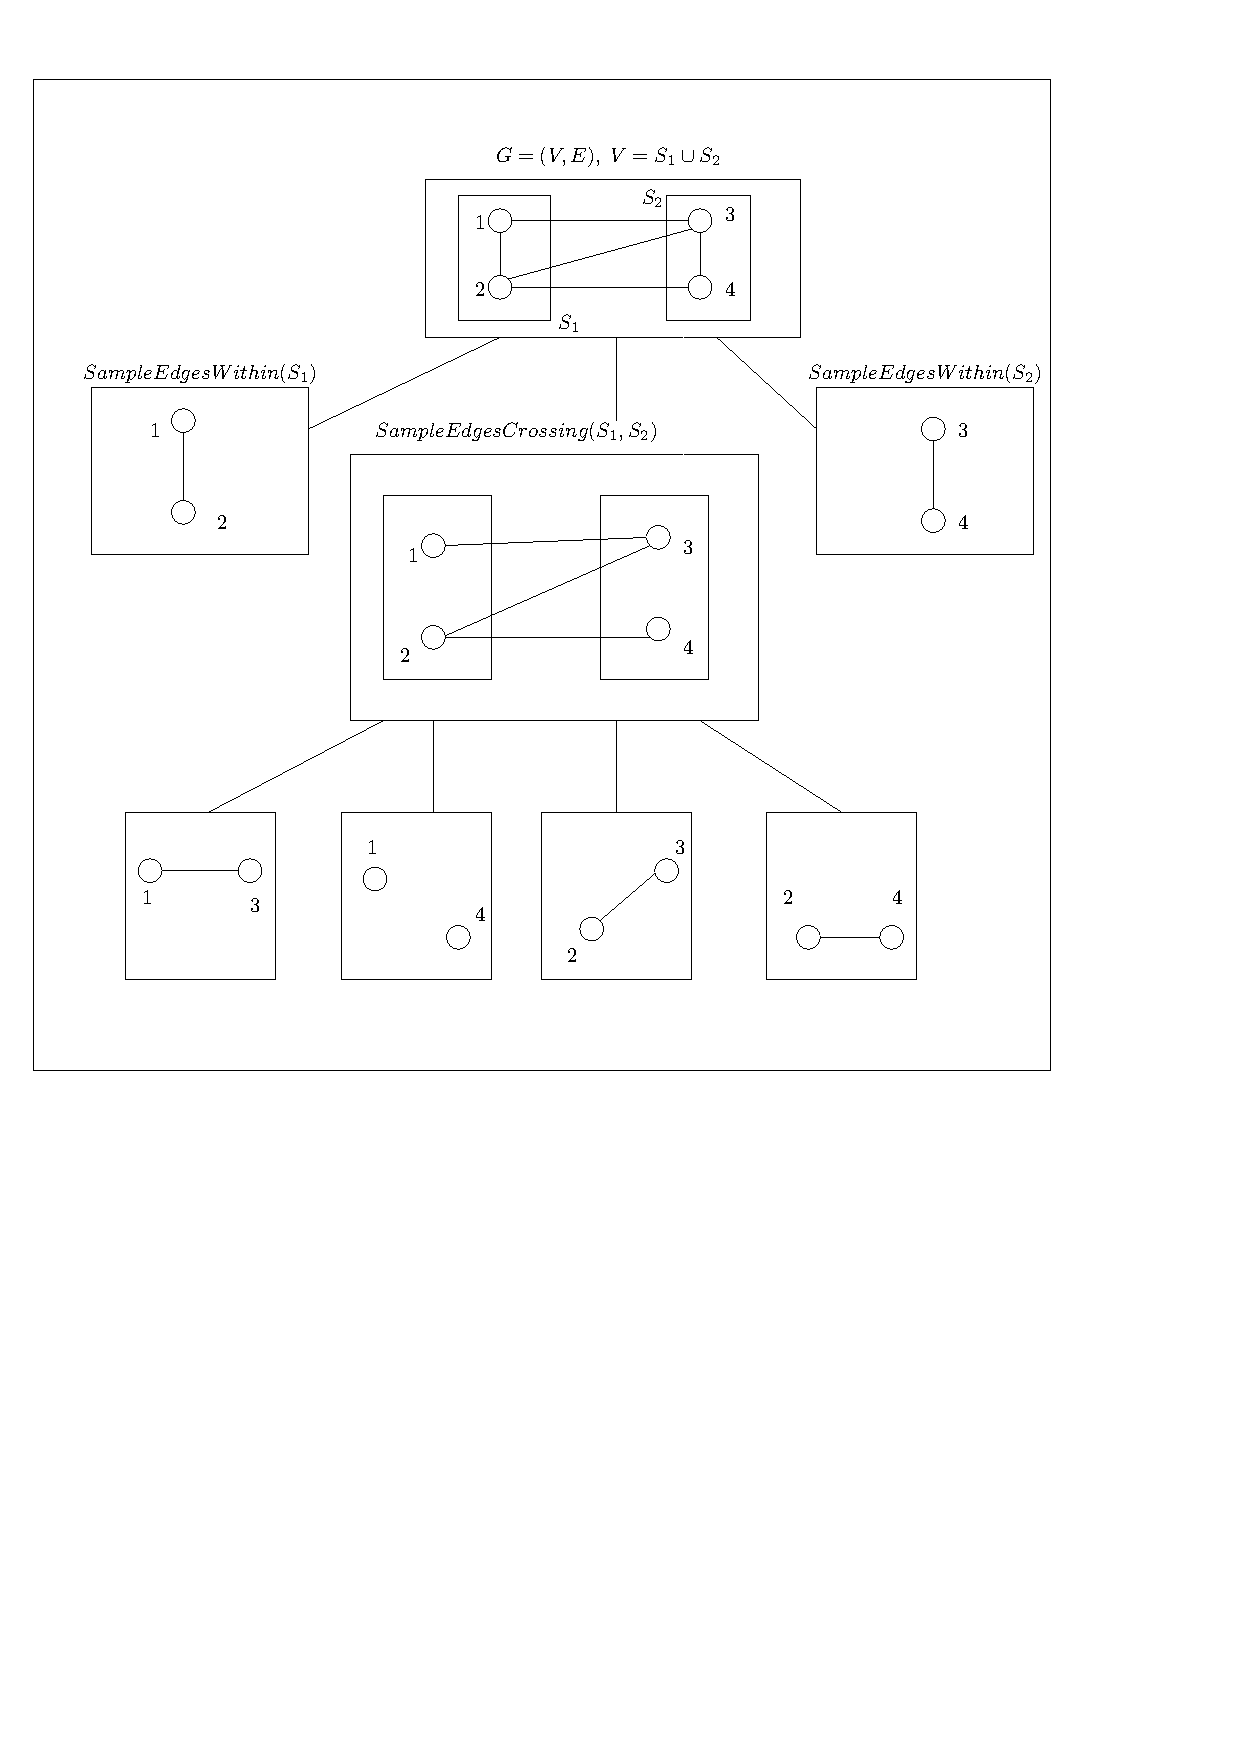
\includegraphics{Figures/alg-tree}
\end{center}


%----------------------------------------------------------------------------------------





